\documentclass[aspectratio=1610]{beamer}
\usetheme{boxes}
\usecolortheme{crane}
\usepackage{amsmath,amsfonts}
\usepackage{algpseudocode}
\usepackage{multicol}
\usepackage{pgfplots}
\pgfplotsset{compat=1.15}
\usepackage{mathrsfs}
\usetikzlibrary{arrows}


%-------------------------------------------------------------------
%	 TITLE SLIDE
%-------------------------------------------------------------------


\begin{document}

% -------------------------------------------------------------------
% Lesson 5
% -------------------------------------------------------------------
\section{Data Pipelines}

\begin{frame}
\begin{center}
\Huge Lesson 5\\~\\
\textbf{Data Pipelines}
\end{center}
\end{frame}


\begin{frame}
\frametitle{Lesson 5}
\Huge In this lesson we will talk about:\\
\huge
 \alert{Data pipelines. Origins and Definitions}\\
 \alert{Data Capture, Transforming \& Analysing}\\
 \alert{Raw Data. Data Aggregation}\\
 \alert{Pipeline efficiency}\\
 \alert{Basic statistical functions}
\end{frame}




\begin{frame}{Lesson 5}{}
\Huge
 What is a data pipeline?
 \end{frame}



\begin{frame}{Lesson 5}{}
\LARGE
Data Pipeline deals with information that is flowing from one end to 
another. In simple words, we can say collecting the data from various 
resources than processing it as per requirement and transferring it 
to the destination by following some sequential activities.\\~\\
Source: www.geeksforgeeks.org
\end{frame}

\begin{frame}[plain,noframenumbering]
\makebox[\linewidth]{\includegraphics[width=\paperwidth]{Images/pipeline1}}
\end{frame}



\begin{frame}{Lesson 5}{}
\LARGE
A data pipeline is a method in which raw data is ingested from 
various data sources, transformed and then ported to a data store, 
such as a data lake or data warehouse, for analysis.
\end{frame}

\begin{frame}{Lesson 5}{}
\LARGE
Data pipelines act as the “piping” for data science projects or 
business intelligence dashboards. Data can be sourced through a wide 
variety of places: APIs, SQL and NoSQL databases, files.
\end{frame}

\begin{frame}{Lesson 5}{}
\LARGE
During sourcing, data lineage is tracked to document the relationship 
between enterprise data in various business and IT applications, for 
example, where data is currently and how it’s stored in an 
environment, such as on-premises, in a data lake or in a data 
warehouse.\\~\\
Source: ibm.com
\end{frame}


\begin{frame}{Lesson 5}{}
\LARGE
A data pipeline is a series of processing steps to prepare enterprise 
data for analysis. Organizations have a large volume of data from 
various sources like applications, Internet of Things (IoT) devices, 
and other digital channels. However, raw data is useless; it must be 
moved, sorted, filtered, reformatted, and analyzed for business 
intelligence. A data pipeline includes various technologies to 
verify, summarize, and find patterns in data to inform business 
decisions.\\~\\
Source: amazon.com
\end{frame}


\begin{frame}[plain,noframenumbering]
\makebox[\linewidth]{\includegraphics[width=\paperwidth]{Images/pipeline1}}
\end{frame}



\begin{frame}
\begin{center}
\Huge
\begin{quote}
\textbf{"A pipeline is a mechanism for connecting the output of one program directly and conveniently into the 
    input of another program."}
\begin{flushright}
{--- Brian Kernighan, UNIX father}	
\end{flushright}
\end{quote}
\end{center}
\end{frame}



\begin{frame}[plain,noframenumbering]
\makebox[\linewidth]{\includegraphics[width=\paperwidth]{Images/pipeline}}
\end{frame}


\begin{frame}{Lesson 5}{}
\Huge
 Our software is \textbf{complex}, \textbf{buggy} and \textbf{difficult} to maintain.
 \end{frame}


\begin{frame}
\begin{center}
\Huge
\begin{quote}
\textbf{"If our software is buggy, what does
that say about its security?"}
\begin{flushright}
{--- Prof. Robert H. Morris}
\end{flushright}
\end{quote}
\end{center}
\end{frame}


\begin{frame}[plain,noframenumbering]
\makebox[\linewidth]{\includegraphics[width=\paperwidth]{Images/outage1}}
\end{frame}

\begin{frame}[plain,noframenumbering]
\makebox[\linewidth]{\includegraphics[width=\paperwidth]{Images/outage2}}
\end{frame}

\begin{frame}[plain,noframenumbering]
\makebox[\linewidth]{\includegraphics[width=\paperwidth]{Images/outage3}}
\end{frame}

\begin{frame}{Lesson 2}{}
\Huge
\center
    \textbf{What can we do about it?} 
\end{frame}



\begin{frame}{Lesson 2}{}
\Huge
\begin{center}
   Start with a \textbf{smart design} at the specification level
\end{center}
\end{frame}


\begin{frame}{Lesson 2}{}
\begin{center}
\Huge\textbf{Software Specifications}
\end{center}
\end{frame}


\begin{frame}{Lesson 2}{}
\Huge{What is a specification?}
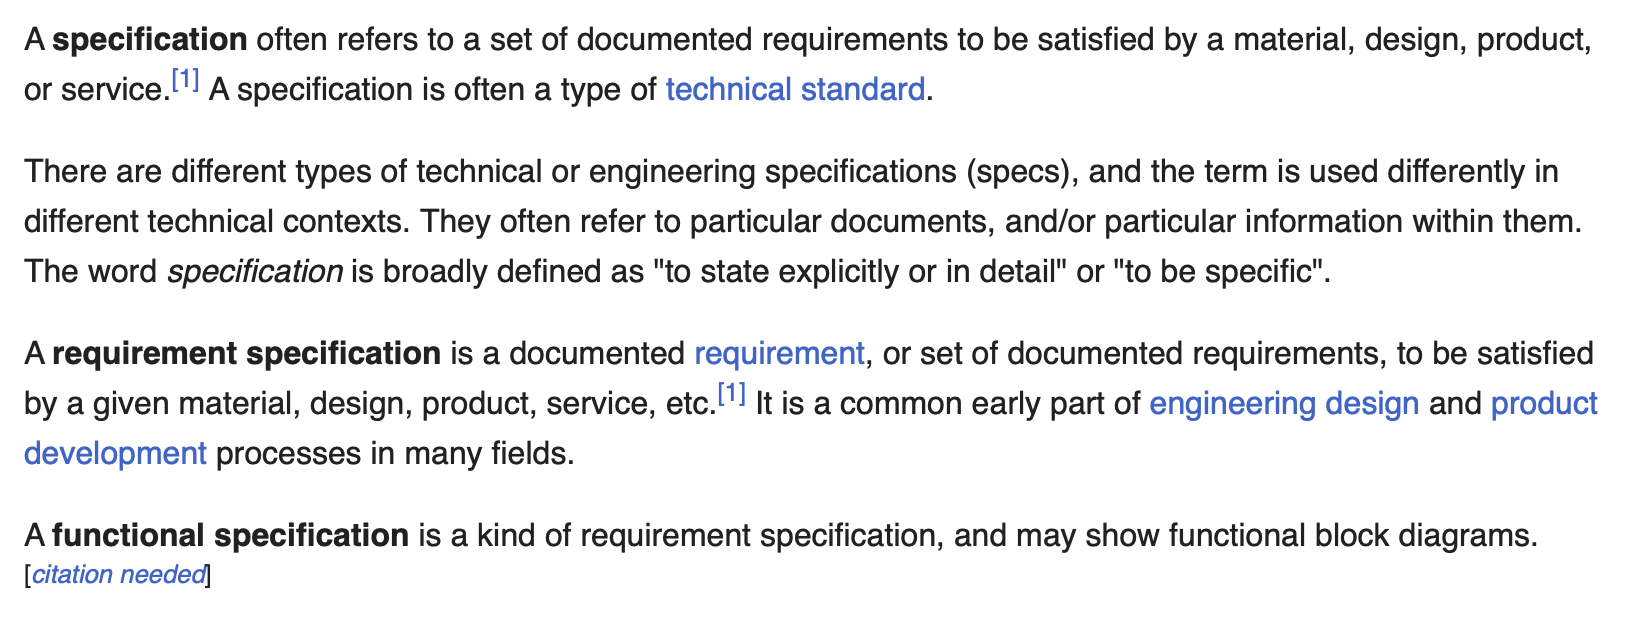
\includegraphics[scale=0.52]{Images/specs}
\end{frame}


\begin{frame}{Lesson 2}{}
\Huge{What is a functional specification?}
\includegraphics[scale=0.46]{Images/funcspecs0}
\end{frame}


\begin{frame}{Lesson 2}{}
\huge
    A \textbf{functional software specification} is a
    \alert{written} description of what our program is supposed to do.
\end{frame}


\begin{frame}{Lesson 2}{}
\includegraphics[scale=0.41]{Images/funcspecs}
\end{frame}



\begin{frame}{Lesson 2}{}
\LARGE
\textbf{How can we write the specification?}\\~\\
\begin{itemize}
    \item English. Finnish. Chinese
    \item Graphical diagrams. Drawing
    \item Technical sketches. Mockups
\end{itemize}
\end{frame}


\begin{frame}{Lesson 2}{}
\LARGE
\textbf{Functional specification}\\~\\
Helps us to understand what our program will do. It’s highly important to write first a specification of our program \alert{before}  implementing and developing anything.
\end{frame}




\begin{frame}{Lesson 2}{}
\LARGE
    \textbf{The specification -- what our program does.}\\~\\
  
\textbf{But how should we describe this specification? How can we be precise? What does it mean to be precise?}
\end{frame}



\begin{frame}{Lesson 2}{}
\begin{center}
\Huge
	Imprecision can lead to \alert{\textbf{ERRORS!}}
\end{center}
\end{frame}


\begin{frame}{Lesson 2}{}
\LARGE
\textbf{Precise specifications}\\~\\
Its difficult to be precise using English or Chinese. Thats why in science and engineering precise specifications have adopted basic maths to describe the specifications.
\end{frame}


\begin{frame}{Lesson 2}{}
\LARGE
\textbf{Basic math}\\~\\
Elementary mathematics. Propositional logic.
\end{frame}


\begin{frame}{Lesson 2}{}
\LARGE
\textbf{Propositional Logic}\\~\\
\includegraphics[scale=0.54]{Images/basiclogic}
\end{frame}


\begin{frame}{Lesson 2}{}
\LARGE
\textbf{Propositional Logic, cont.}
\includegraphics[scale=0.55]{Images/basiclogic2}
\end{frame}



\begin{frame}{Lesson 2}{}
\LARGE
\textbf{Formal methods}\\~\\
\includegraphics[scale=0.53]{Images/fm}
\end{frame}


\begin{frame}{Lesson 2}{}
\LARGE
\textbf{Specifications using formal methods}\\~\\
\includegraphics[scale=0.53]{Images/fms}
\end{frame}


\begin{frame}{Lesson 2}{}
\LARGE
    Formal verification is the use of software tools to prove properties of a formal specification, or to prove that a formal model of a system implementation satisfies its specification.\\~\\
\textbf{Once a formal specification has been developed, the specification may be used as the basis for proving properties of the specification.}
\end{frame}

\begin{frame}{Lesson 2}{}
\LARGE
\textbf{Why maths?}\\~\\
\begin{itemize}
    \item Quantify output behavior
    \item Predict behavior of systems as design time
    \item Understand safety margins
    \item Understand system interactions
\end{itemize}
\end{frame}


\begin{frame}{Lesson 2}{}
\LARGE
    \textbf{Verification: Are we building the product right?}

\end{frame}

\begin{frame}{Lesson 2}{}
\LARGE
    \textbf{Validation: Are we building the right product?}
\end{frame}

\begin{frame}{Lesson 2}{}
\LARGE
"Building the product right" checks that the specifications are correctly implemented by the system while "building the right product" refers back to the user's needs. Ideally, formal methods provide a mathematical guarantee that software meets its specifications.
\end{frame}


\begin{frame}{Lesson 2}{}
	\Huge Industry
\end{frame}


\begin{frame}[plain,noframenumbering]
\makebox[\linewidth]{\includegraphics[width=\paperwidth]{Images/fmaws2}}
\end{frame}

\begin{frame}{Lesson 2}{}
\LARGE
\textbf{Industry: Amazon, Microsoft, NASA, ESA, Intel}\\~\\
\includegraphics[scale=0.18]{Images/fmaws}
\includegraphics[scale=0.25]{Images/fmms}
\end{frame}





%\begin{frame}{Lesson 2}{}
%\LARGE
%\textbf{}\\~\\
%A computer system differs from the systems traditionally studied by 
% scientists because we can
%pretend that its state changes in discrete steps. So, we represent the 
%execution
%of a system as a sequence of states. Formally, we define a behavior to be 
%a
%sequence of states, where a state is an assignment of values to 
%variables. We
%specify a system by specifying a set of possible behaviors—the ones 
%representing
%a correct execution of the system

\end{document}

